\newpage
\part{Morpion et Monte Carlo}
\section{Description du problème}
Dans cette partie, on considère le célèbre jeu du Tic Tac Toe qui se joue sur une grille 3$\times$3. Les joueurs alternent tour à tour en plaçant un «X» ou un «O» sur une case vide de la grille. Le premier joueur à aligner trois symboles gagne. Nous allons considérer deux types de joueurs, des joueurs $Random$ qui se contenteront de choisir leurs prochains coups à jouer aléatoirement et des joueurs qui, eux, utiliseront une méthode de $Monte$ $Carlo$.
L'implémentation de ce jeu est basée sur quatre classes : \verb@State@ qui représente l'état du jeu, une classe \verb@Agent@ qui elle, représente le comportement d'un agent. La méthode \verb@get_action@ permet à l'agent de  

\section{Joueur Aléatoire}
\begin{figure}[ht]
\centering
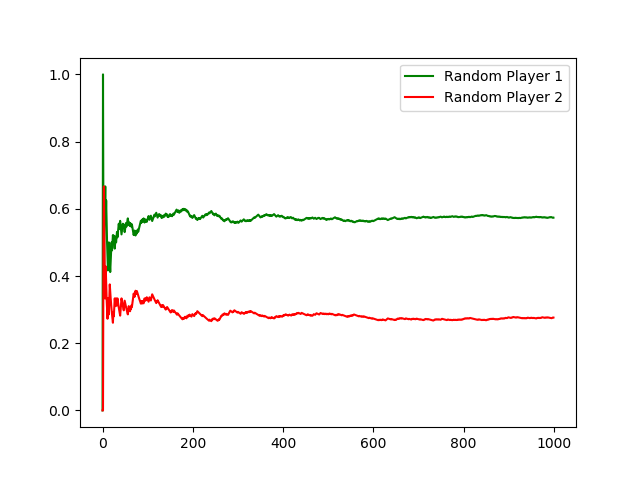
\includegraphics[width=0.6\textwidth]{Report/sections/Figures/Figure15.png}
\caption{Espérance de gain pour deux joueurs $Random$}
\label{FigGraphes}
\end{figure}
La stratégie aléatoire consiste à exploiter que les actions possibles comme information sur le jeu
On considère une partie comme étant une expérience à deux issus : victoire ou défaite du Joueur 1.
On note $X$ la variable aléatoire qui dénote la victoire du Joueur 1, en cas de victoire, on donne à $X$ la valeur 1, sinon elle prend la valeur 0. Il est évident alors que $X$ suit une loi de Bernoulli, sur la figure ci-dessus, on peut déduire visuellement le paramètre $p$, en effet, en moyenne, le Joueur 1 a une probabilité
$\mathbb{P}$($X$=1)=0.6 de gagner. On en déduit que X suit une loi de Bernoulli de paramètre $p$=0.6 et de variance $\mathbb{V}$($X$)= $p$(1-$p$) = 0.24.

\section{Joueur Monte Carlo}
L'idée générale d'une simulation de $Monte$ $Carlo$ consiste à jouer un certain nombre de parties avec des choix aléatoires puis d'utiliser les résultats de ces parties pour calculer une bonne action à jouer. Lorsqu'un joueur gagne une de ces parties aléatoires, il devra privilégier les actions qui l'ont mené à cette victoire, dans l'espoir de choisir un coup gagnant lors des prochaines parties et éviter les actions qui ont mené son adversaire à la defaite. Une stratégie $Monte$ $Carlo$ échantillonne aléatoirement l'espace de toutes les actions possibles et fait une estimation de l'action qui semble la plus optimale.
\subsection{Implémentation}
Pour implémenter cet algorithme nous avons créer une classe \newline\verb@MonteCarloAgent@ qui hérite de \verb@Agent@ et qui implémente la méthode \verb@get_action@ dans laquelle on recupère d'abord toutes les actions possibles ensuite, pour $N$ itérations, on choisit une action aléatoirement, on recupère l'état du jeu qui sera joué après cela par deux joueurs aléatoires, enfin, on met à jour la récompense associée à cet action selon le cas où elle a conduit à une victoire ou une défaite. La méthode renvoie l'action avec la plus grande récompense.
\subsection{Random VS Monte Carlo}
\begin{figure}[htbp]
   \begin{subfigure}[b]{0.47\textwidth}
        \centering 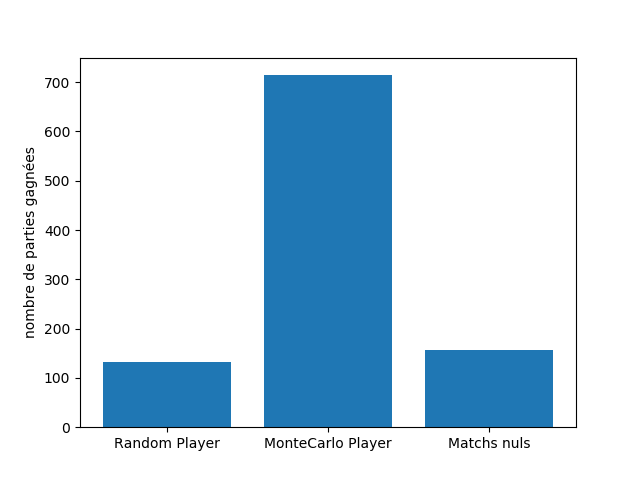
\includegraphics[width=\textwidth]{Report/sections/Figures/Figure16.png}
        \caption{Statistique sur 1000 parties jouées entre un Joueur $Random$ et un Joueur $Monte$ $Carlo$}
    \end{subfigure}
    \begin{subfigure}[b]{0.47\textwidth}
        \centering 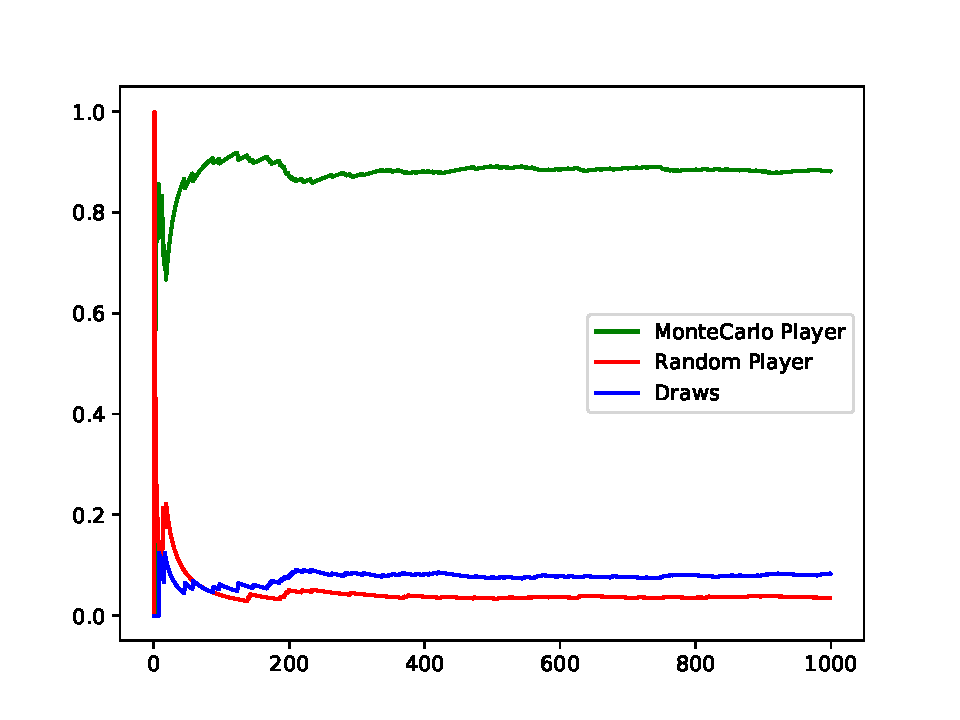
\includegraphics[width=\textwidth]{Report/sections/Figures/Figure17.pdf}
        \caption{Espérance de gain pour chaque joueur}
    \end{subfigure}
    
    \caption{Comparaison entre un Joueur $Random$ et un Joueur $Monte$ $Carlo$}
\end{figure}
On peut observer sur la figure 4 que le joueur basé sur la méthode de $Monte$ $Carlo$ surpasse largement le joueur $Random$ en terme de parties gagnées. Cependant, il existe des situations où gagner est impossible pour le joueur $Monte$ $Carlo$, malgré le fait que sa politique de jeu soit plus intelligente que celle du joueur $Random$, par exemple, la défaite est inévitable si c'est le joueur $Random$ qui entame la partie et qu'il marque la case centrale en premier, dans ce cas, beaucoup de voies seront bloquées dans la grille et donc peu importe la stratégie du joueur, cela ne lui évitera pas la défaite.
\newpage
\subsection{Monte Carlo VS Monte Carlo}
La figure 5 ci-dessous illustre très bien l'avantage donné au joueur qui entame la partie étant donnée que son espérance de gain est plus elevée que celle du joueur adverse bien qu'ils suivent la meme stratégie de jeu. Cela peut s'expliquer, comme précédemment, par le fait qu'il est presque impossible de gagner pour un joueur lorsqu'il n'entame pas la partie.
\begin{figure}[ht]
\centering
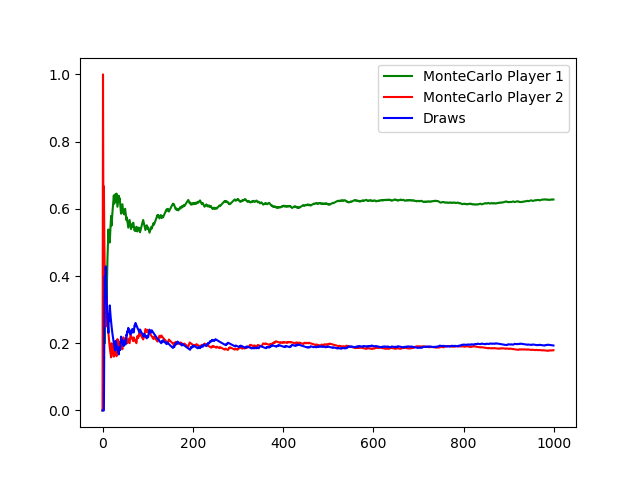
\includegraphics[width=0.6\textwidth]{Report/sections/Figures/Figure13.png}
\caption{Espérance de gain pour deux joueurs $Monte$ $Carlo$}
\label{FigGraphes}
\end{figure}
\newpage
